\section[Lezione 23 - MEG e soluzioni di sistemi lineari]{Lezione 23 - MEG e soluzione di sistemi lineari: sistemi triangolari, uso della fattorizzazione LU, inversione di matrici, MEG e condizionamento}
Nelle ultime due lezioni abbiamo studiato il meg come metodo per la riduzione di una matrice non singolare a forma triangolare (superiore) e in ultima analisi come metodo per la fattorizzazione LU (prodotto di una triangolare inferiore per una triangolare superiore) nella forma
\begin{center}
    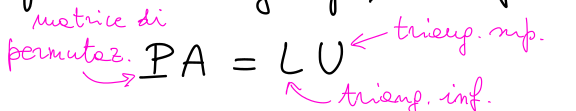
\includegraphics[scale=0.5]{foto/pag1}
\end{center}
In questa lezione vedremo come usare la fattorizzazione LU per risolvere un sistema lineare con $A$ non singolare
\begin{equation*}
    Ax=b, \ det(A)\neq 0
\end{equation*}
Ricordiamo l'\uline{approccio standard} per la soluzione di un sistema col meg: si aggiunge ad $A$ una colonna uguale al vettore termine noto $b$ e si applicano le trasformazioni che portano alla forma triangolare superiore a questa matrice ``orlata"$\in \mathbb{R}^{n \times (n+1)}$
\begin{equation*}
    \begin{split}
        & [A^{(1)}|b^{(1)}] = [A|b]\rightarrow [A^{(2)}|A^{(2)}] \rightarrow \\
        & ... \rightarrow [A^{(n)}|b^{(n)}] = [U|\beta]
    \end{split}
\end{equation*}
Cioè le trasformazioni (scambi di righe dovuti al pivoting e combinazioni di righe per gli annullamenti sotto la diagonale principale) vengono applicate anche al vettore termine noto, ottenendo alla fine un sistema triangolare superiore
\begin{equation*}
    Ux=\beta
\end{equation*}
Questo sistema è equivalente al sistema di partenza $Ax=b$, nel senso che hanno la stessa soluzione: infatti in generale moltiplicare un sistema $Bx=c$ a sinistra per una matrice invertibile (come sono le matrici elementari di trasformazione)
\begin{equation*}
    EBx = Ec, \ det(E) \neq 0
\end{equation*}
non cambia le soluzione, perché se $Bx=c$ allora $EBx=Ec$ e se $EBx=Ec$ allora $E^{-1}EBx = Bx = E^{-1}Ec = c$

\subsection{Soluzione di $Ux=\beta$}
Una volta ottenuto il sistema equivalente $Ux=\beta$, questo può essere facilmente risolto col metodo detto della ``SOSTITUZIONE ALL'INDIETRO" (BACKWARD SUBSTITUTION in inglese), che richiameremo ora brevemente. \\
Scrivendo $Ux=\beta$ in forma estesa
\begin{equation*}
    \begin{pmatrix}
        u_{11} & u_{12} & \dots & u_{1n-1} & u_{1n} \\ 
        & u_{22} & \dots & u_{2n-1} & u_{2n} \\ 
        & \ddots &  & \vdots & \vdots \\ 
        &  & \ddots  & u_{n-1n-1} & u_{n-1n} \\ 
        &  &  &  & u_{nn} 
    \end{pmatrix} 
    \begin{pmatrix}
        x_1 \\ 
        x_2 \\ 
        \vdots \\ 
        x_{n-1} \\ 
        x_n 
    \end{pmatrix} = 
    \begin{pmatrix}
        \beta_1 \\ 
        \beta_2 \\ 
        \vdots \\ 
        \beta_{n-1} \\ 
        \beta_n 
    \end{pmatrix}
\end{equation*}
cioè
\begin{equation*}
    \begin{cases}
u_{11}x_1 +u_{12}x_2 + \dots + u_{1n-1}x_{n-1} + u_{1n}x_n = \beta_1\\ 
 u_{22}x_2 + \dots +u_{2n-1}x_{n-1} + u_{2n}x_n = \beta_2\\ 
\vdots  \\ 
 u_{n-1n-1}x_{n-1} + u_{n-1n}x_n = \beta_{n-1}\\ 
 u_{nn}x_n = \beta_{n}
\end{cases}
\end{equation*}
dove $u_{ii}\neq 0 \ \forall i$.\\
E' evidente che l'ultima equazione ha una sola incognita, quindi 
\begin{equation*}
    x_n = \frac{\beta_n}{u_{nn}}
\end{equation*}
Questo valore può allora essere sostituito nella penultima equazione, che diventa nella sola incognita $x_{n-1}$,
\[
u_{n-1n-1}x_{n-1}+u_{n-1n}\overset{=\beta_n/u_{nn}}{x_n}=\beta_{n-1}
\]
da cui 
\[x_{n-1}=\frac{1}{u_{n-1n-1}}(\beta_{n-1}-u_{n-1n}\overset{=\beta_n/u_{nn}}{x_n})
\]
Questo procedimento si può ripetere con le righe $n-2$, $n-3$,..., 2, 1 fino a calcolare tutte le incognite. Al passo $i$-esimo
\begin{equation*}
    x_i = \frac{1}{u_{ii}} \biggl( \beta_i - \sum_{j=i+1}^n u_{ij}x_j \biggr), \ i=n,n-1,\dots,1
\end{equation*}
dove i valori $x_j$, $j=i+1,...,n$ sono stati calcolati ai passi precedenti (ponendo $\sum_{j=n+1}^n = 0$ in modo che la formula sia valida anche per $i=n$). \\
Possiamo calcolare facilmente il \uline{costo computazionale} della sostituzione all'indietro: ci sono infatti $n$ divisioni e ad ogni passo $i=n-1,...,1$ ci sono $n-i$ moltiplicazioni e $n-i$ somme algebriche, quindi in tutto
\begin{equation*}
    \begin{split}
        c_n^{BS} & = n + \sum_{i=1}^{n-1} 2(n-i) \\
                 & = n + 2\sum_{j=1}^{n-1} j \\
                 & = n + 2\frac{n(n-1)}{2} = n^2 \ flops
    \end{split}
\end{equation*}
In definita, il costo computazionale della soluzione di una sistema col meg, per quanto visto nella lezione 21 e tenendo conto del fatto che le trasformazioni vanno applicate anche al vettore termine noto (come colonna $n+1$-esima della matrice orlata), è 
\begin{equation*}
    \begin{split}
        c_n^{Sist1} & = c_n^{meg} + \underbrace{2\sum_{i=1}^{n-1}}_{=\frac{2n(n-1)}{2}\sim n^2} (n-i) + c_n^{BS} \\
        & \sim \frac{2}{3}n^3 + n^2 + n^2 = \frac{2}{3}n^3 + 2n^2 \ flops
    \end{split}
\end{equation*}
cioè il termine dominante resta cubico (ma abbiamo meno in evidenza i costi asintotici del calcolo di $\beta$ e della sostituzione all'indietro). \\
Scopriremo tra poco che può essere vantaggioso risolvere $Ax=b$ col meg tramite la fattorizzazione LU

\subsection{Sistemi lineari via LU}
Oltre all'approccio standard appena descritto, esiste un altro modo di usare il meg per risolvere sistemi lineari, passando per la fattorizzazione LU. \\
Consideriamo infatti un sistema
\begin{equation*}
    Ax=b, \ det \neq 0
\end{equation*}
e supponiamo di aver applicato il meg (con pivoting) ad $A$ ottenendo
\begin{equation*}
    PA = LU
\end{equation*}
Il sistema di partenza evidentemente è equivalente al sistema
\begin{equation*}
    PAx=LUx=\uline{P}b
\end{equation*}
visto che la matrice di permutazione $\uline{P}$ è invertibile (essendo prodotto di matrici di scambio che sono invertibili). \\
Una volta calcolare $L$ ed $U$, che come sappiamo vengono prodotte dal meg, come possiamo risolvere il sistema $LUx=\uline{P}b$?\\
E' equivalente risolvere in cascata la coppia di sistemi
\begin{equation*}
    \begin{cases}
         & Ly = \uline{P}b \\
         & Ux = y
    \end{cases}
\end{equation*}
che sono sistemi triangolari! \\
Abbiamo visto sopra come risolvere un sistema triangolare superiore (non singolare) con la sostituzione all'indietro. \\
Analogamente un sistema triangolare inferiore si può risolvere con la ``SOSTITUZIONE IN AVANTI" (FORWARD SUBSTITUTION in inglese). \\
Partiamo dalla forma estesa di $Ly = c$
\begin{equation*}
    \begin{pmatrix}
        l_{11} & & & \\
        l_{21} & l_{22} & & \\
        \vdots & \vdots & \ddots & \\
        l_{n1} & l_{n2} & \dots & l_{nn} 
    \end{pmatrix}
    \begin{pmatrix}
        y_1\\
        y_2 \\
        \vdots \\
        y_n 
    \end{pmatrix} = 
    \begin{pmatrix}
        c_1\\
        c_2 \\
        \vdots \\
        c_n 
    \end{pmatrix}
\end{equation*}
cioè
\begin{equation*}
    \begin{cases}
    l_{11}y_1 = c_1\\ 
    l_{21}y_2 + l_{22}y_2 = c_2 \\ 
    \vdots\\ 
    l_{n1}y_1 +l_{n2}y_2 + \dots + l_{nn}y_{n} = c_n
\end{cases}
\end{equation*}
dove $l_{ii}\neq 0 \ \forall i$ ($L$ non singolare). \\
Nella prima equazione compare la sola incognita $y_1$, $y_1 = \frac{c_1}{l_11}$ che sostituita nella seconda permette di ricavare $y_2=\frac{1}{l_{22}}(c_2 - l_{21}y_1)$ e così via in avanti fino all'ultima equazione. \\
Al passo $i$-esimo in formule
\begin{equation*}
    y_i = \frac{1}{l_{ii}}\biggl( c_i - \sum_{j=1}^{i-1} l_{ij}y_j \biggr), \ i=1,\dots,n
\end{equation*}
(ponendo $\sum_{j=1}^0 = 0$ in modo che la formula sia valida anche per $i=1$).\\
Il costo computazionale è lo stesso della sostituzione all'indietro ed è 
\begin{equation*}
    c_n^{FS} = n^2 \ flops
\end{equation*}
Quindi il costo della soluzione di un sistema via meg e $LU$ è 
\begin{equation*}
    c_n^{Sist2} = c_n^{meg} + c_n^{FS} + c_n^{BS} \sim \frac{2}{3}n^3 + 2n^2 \ flops
\end{equation*}
Si noti che questo coincide con il costo della soluzione standard via meg: ciò non è affatto sorprendente, perché in realtà il vettore $y$ soluzione di $Ly=b$ è $y=\beta$, cioè coincide con il risultato delle trasformazioni del meg applicate all'ultima colonna della matrice orlata $[A|b]\in \mathbb{R}^{n\times (n+1)}$. \\
In pratica, è solo un modo di calcolare $\beta$ a posteriori dopo aver ridotto $A$ a forma triangolare superiore e aver calcolato i moltiplicatori.\\
Ma visto che le due procedure sono equivalenti, quando può convenire risolvere un sistema via $LU$? \\
Una situazione di interesse pratico in molte applicazioni è quella in cui si debbano risolvere diversi sistemi, tutti con la stessa matrice non singolare $A$, in cui varia il vettore termine noto
\begin{equation*}
    Ax^{(k)} = b^{(k)}, \ 1 \leq k \leq M
\end{equation*}
in particolare quando $M$ è grande.\\
In queste situazioni non ha molto senso applicare $M$ volte il metodo standard, cioè
\begin{equation*}
    [A|b] \overset{meg}{\longrightarrow} [U|\beta] \overset{BS}{\longrightarrow} x^{(k)}
\end{equation*}
per $k=1,...,M$, perché il costo sarebbe
\begin{equation*}
    c_n^{(1)} \sim \frac{2}{3}n^3M \ flops
\end{equation*}
Invece è molto più efficiente calcolare una volta per tutte la fattorizzazione $\uline{P}A=LU$ (col meg a costo $\sim \frac{2}{3}n^3$) e poi risolvere la sequenza di $M$ sistemi tringolari accoppiati
\begin{equation*}
    \begin{cases}
        & Ly^{(k)} = \uline{P}b^{(k)} \\
        & Ux^{(k)} = y^{(k)}
    \end{cases}
\end{equation*}
con un costo complessivo in flops
\begin{equation*}
    c_n^{(2)} \sim \frac{2}{3}n^3 + 2n^2M \ll \frac{2}{3}n^3M \sim c_n^{(1)}
\end{equation*}
perché il fattore $M$ moltiplica il termine quadratico e non quello cubico!\\
Un esempio interessante in cui si può applicare convenientemente questo approccio è quello della

\subsection{Inversione di matrici}
Anche se il calcolo esplicito dell'inversa $A^{-1}$ di una matrice non singolare $A$ tipicamente non viene fatto per risolvere un sistema (si preferisce applicare un metodo specifico, ad es. il meg), ci sono applicazioni in cui può essere importante avere a disposizione la matrice inversa. \\
Un modo semplice per calcolare l'inversa si basa su una proprietà del prodotto matrice-vettore che abbiamo usato spesso, cioè che $z=Bc$ si può interpretare come combinazione lineare delle colonne di $B$ tramite i coeff, di $c$, cioè
\begin{equation*}
    z=Bc=c_1\underset{\text{colonna 1 di $B$}}{C_1(B)}+\dots+c_n\underset{\text{colonna $n$ di $B$}}{C_n(B)}
\end{equation*}
Se applichiamo questa osservazione con
\begin{equation*}
    c=e^{(i)}=\begin{pmatrix}
    0 \\
    \vdots \\
    0 \\
    1 \\
    0 \\
    \vdots \\
    0
    \end{pmatrix}
\end{equation*}
cioè $c_i = 1$ e $c_j = 0$, $j \neq i$, otteniamo
\begin{equation*}
    Be^{(i)} = C_i(B)
\end{equation*}
Allora per $B=A^{-1}$
\begin{equation*}
    C_i(A^{-1})=A^{-1}e^{(i)} \Leftrightarrow AC_i(A^{-1})=e^{(i)}
\end{equation*}
cioè $C_i(A^{-1})$ è la soluzione di
\begin{equation*}
    Ax^{(i)} = e^{(i)}, \ 1\leq i \leq n
\end{equation*}
Possiamo quindi calcolare l'inversa ``per colonne" risolvendo $M=n$ sistemi lineari, tutti con matrice $A$, in cui il termine noto varia tra gli $n$ vettori coordinati della base canonica. \\
Se usassimo $n$ volte il metodo standard avremmo un costo
\begin{equation*}
    c_n^{(1)} \sim \frac{2}{3}n^3M = \frac{2}{3}n^4 \ flops
\end{equation*}
Invece calcolando una volta col meg la fattorizzazione LU e risolvendo le $M=n$ coppie di sistemi triangolari
\begin{equation*}
    \begin{cases}
        & Ly^{(i)} = \uline{P}e^{(i)} \\
        & Ux^{(i)} = y^{(i)}
    \end{cases}
\end{equation*}
si ha un costo 
\begin{equation*}
    c_n^{(2)} \sim \frac{2}{3}n^3 + 2n^2n = \frac{8}{3}n^3 \ flops
\end{equation*}
cioé l'\uline{inversa} si può calcolcare col \uline{meg} (via LU) a \uline{costo cubico} nella dimensione (e questo è in sostanza il metodo che usano tutti i sistemi di calcolo, ad es. il Matlab, quando si usa una function predefinita tipo ``inv(A)").\\
Concludiamo la lezione discutendo, anche tramite un classico esempio, l'effetto del condizionamento di $A$ nella soluzione di $Ax=b$ col meg.

\subsection{MEG e condizionamento}
In questo paragrafo discutiamo l'effetto del condizionamento della matrice $A$ sul meg, implementato in aritmetica floating-point, nella soluzione di $Ax=b$ (via fattorizzazione LU, che comunque è equivalente al metodo standard dal punto di vista dei calcoli coinvolti). \\
Ci sono in realtà 2 aspetti legati alla stabilità del meg per quanto riguarda la propagazione degli errori di arrotondamento.\\
Il primo aspetto è la potenziale instabilità dovuta alla generazione di numeri arrotondati sempre più grandi in assenza di controllo sull'elemento diagonale usate per gli allunamenti in colonna. \\
Questo problema viene risolto come abbiamo già osservato dal \uline{pivoting}, che ha un effetto stabilizzante sull'algoritmo. \\
Dal punto di vista del meg come algoritmo di fattorizzazione, si vede in pratica che col pivoting la fattorizzazione è estremamente accurata, nel senso che gli errori di arrotondamento si propagano bene e si ha tipicamente che $\uline{P}A$ è vicinissima ad $LU$ in termini relativi, ad es. in norma-2 indotta
\begin{equation*}
    \frac{\norma{\uline{P}A-LU}_2}{\norma{\uline{P}A}_2} \approx \varepsilon_M
\end{equation*}
Ma quando si va a risolvere un sistema, come sappiamo l'instabilità è a monti cioè viene dal problema se $A$ è mal condizionata.\\
Consideriamo un esempio classico, ovvero la ``matrice di Hilbert"
\begin{equation*}
    H_n=\begin{pmatrix}
        1 & \frac{1}{2} & \frac{1}{3} & \dots & \frac{1}{n} \\ 
        \frac{1}{2} & \frac{1}{3} & \frac{1}{4} & \dots & \frac{1}{n+1} \\ 
        \vdots &  &  &  &  \\ 
        \frac{1}{n} & \frac{1}{n+1} & \frac{1}{n+2} & \dots & \frac{1}{2n-1}
    \end{pmatrix}
\end{equation*}
ovvero $(H_n)_{ij} = \frac{1}{i+j-1}$, $1\leq i,j \leq n$. \\
Si ha che $H_n$ è evidentemente simmetrica ed è anche definita positiva (accettiamo questo fatto). \\
Se applichiamo il meg ad $H_n$, essendo definita positiva il pivoting non agisce perché come abbiamo già ricordato in questo caso il pivoting è sempre sulla diagonale durante il processo di eliminazione (anche questo risultato lo accettiamo) \\
Usando la function ``lu" del Matlab (che usa il meg con pivoting) si ottiene con $n=13$
\begin{equation*}
    \frac{\norma{H_{13}-\Tilde{L}\Tilde{U}}_2}{\norma{H_{13}}_2} \approx 3.6\cdot 10^{-17}
\end{equation*}
dove $\Tilde{L}$ e $\Tilde{U}$ sono i fattori tringolari calcolari in precisione doppia. Invece risolvendo il sistema $H_{13}x=b=H_{13}u$ con $u=\biggl(\begin{smallmatrix} 1 \\ \vdots \\ 1 \end{smallmatrix}\biggr) \in \mathbb{R}^{13}$ la cui soluzione esatta per costruzione $x=u$, detta $\Tilde{x}=x+\delta x$ la soluzione calcolata in Matlab
\begin{equation*}
    \frac{\norma{\Tilde{x}-x}_2}{\norma{x}_2}=\frac{\norma{\delta x}_2}{\norma{x}_2} \approx 17.2
\end{equation*}
cioè si fa un errore relativo $>1000\%$! \\
Perché accade questo?\\
La spiegazione sta nell'indice di condizionamento di $H_n$, che ha una crescita esponenziale in $n$, ad es. $K_2(H_4)\approx 1.6 \cdot 10^4$, $K_2(H_8) \approx 1.5\cdot 10^{10}$, $K_2(H_{12}) \approx 1.6 \cdot 10^{16}$ (è stato dimostrato che $K_2(H_n)$ cresce proporzionalmente a $\frac{(1+\sqrt{2})^{4n}}{\sqrt{n}} \approx \frac{34^n}{\sqrt{n}}$). \\
Infatti risolvere il sistema col meg corrisponde in ultima analisi a risolvere il sistema
\begin{equation*}
    \Tilde{H}_{13}\Tilde{x} = \Tilde{L}\Tilde{U}\Tilde{x}=b
\end{equation*}
Ricordando la stima (lezione 20)
\begin{equation*}
    \frac{\norma{\delta x}}{\norma{\Tilde{x}}} \leq K(A) \frac{\norma{\delta A}}{\norma{A}}
\end{equation*}
ci si può aspettare una potenziale amplificazione di $\frac{\norma{\delta H_{13}}_2}{\norma{H_{13}}_2} \approx 3.6 \cdot 10^{-17}$ di un fattore $K_2(H_{13}) \approx 4.8 \cdot 10^{17}$, che spiega molto bene la perdita di tutta la precisione. \\Con matrici così fortemente mal condizionate, ci sono 2 possibili strade: o si lavori in precisione estesa (ad es. col meg in precisione quadrupla ci si aspetta $\frac{\norma{\delta H_{13}}_2}{\norma{H_{13}}_2} \approx  10^{-32}$ e quindi un errore sulla soluzione $K_2(H_{13}) \cdot 10^{-32} \approx 10^{-15}$) oppure, soprattutto se sono presenti altre fonti di errore oltre agli arrotondamenti (ad esempio errori di misura sperimentale), si rinuncia ad usare un metodo standard come il meg e si ricorre invece ad uno degli algoritmi speciali per sistemi mal condizionati, cui abbiamo fatto un breve cenno facoltativo alla fine della lezione 20.
\newpage